%%%%%%%%%%%%%%%%%%%%%%%%%%%%%%%%%%%%%%%%%
% Short Sectioned Assignment
% LaTeX Template
% Version 1.0 (5/5/12)
%
% This template has been downloaded from:
% http://www.LaTeXTemplates.com
%
% Original author:
% Frits Wenneker (http://www.howtotex.com)
%
% License:
% CC BY-NC-SA 3.0 (http://creativecommons.org/licenses/by-nc-sa/3.0/)
%
%%%%%%%%%%%%%%%%%%%%%%%%%%%%%%%%%%%%%%%%%

%----------------------------------------------------------------------------------------
%	PACKAGES AND OTHER DOCUMENT CONFIGURATIONS
%----------------------------------------------------------------------------------------

\documentclass[paper=a4, fontsize=11pt]{scrartcl} % A4 paper and 11pt font size

\usepackage[T1]{fontenc} % Use 8-bit encoding that has 256 glyphs
\usepackage{fourier} % Use the Adobe Utopia font for the document - comment this line to return to the LaTeX default
\usepackage[english]{babel} % English language/hyphenation
\usepackage{amsmath,amsfonts,amsthm} % Math packages
\usepackage{graphicx}
\usepackage{tikz}
\usetikzlibrary{arrows}
\usetikzlibrary{positioning}

\usepackage{lipsum} % Used for inserting dummy 'Lorem ipsum' text into the template

\usepackage{sectsty} % Allows customizing section commands
\allsectionsfont{\centering \normalfont\scshape} % Make all sections centered, the default font and small caps

\usepackage{fancyhdr} % Custom headers and footers
\pagestyle{fancyplain} % Makes all pages in the document conform to the custom headers and footers
\fancyhead{} % No page header - if you want one, create it in the same way as the footers below
\fancyfoot[L]{} % Empty left footer
\fancyfoot[C]{} % Empty center footer
\fancyfoot[R]{\thepage} % Page numbering for right footer
\renewcommand{\headrulewidth}{0pt} % Remove header underlines
\renewcommand{\footrulewidth}{0pt} % Remove footer underlines
\setlength{\headheight}{13.6pt} % Customize the height of the header

\numberwithin{equation}{section} % Number equations within sections (i.e. 1.1, 1.2, 2.1, 2.2 instead of 1, 2, 3, 4)
\numberwithin{figure}{section} % Number figures within sections (i.e. 1.1, 1.2, 2.1, 2.2 instead of 1, 2, 3, 4)
\numberwithin{table}{section} % Number tables within sections (i.e. 1.1, 1.2, 2.1, 2.2 instead of 1, 2, 3, 4)

\setlength\parindent{0pt} % Removes all indentation from paragraphs - comment this line for an assignment with lots of text

%----------------------------------------------------------------------------------------
%	TITLE SECTION
%----------------------------------------------------------------------------------------

\newcommand{\horrule}[1]{\rule{\linewidth}{#1}} % Create horizontal rule command with 1 argument of height

\title
{	
\normalfont \normalsize 

\includegraphics[scale=0.7]{feup.png}
\horrule{0.5pt} \\[0.4cm] % Thin top horizontal rule
\huge Project Management with Computational Trust Models in a Multi-Agent Environment\\
\horrule{2pt} \\[0.5cm] % Thick bottom horizontal rule
}

\author{
	Ricardo Ferreira da Silva\\
	\texttt{up201305163@fc.up.pt}
	\and
	Gustavo de Castro Nogueira Pinto\\
	\texttt{up201302828@fe.up.pt}
	\and
	Tiago Filipe Abreu Figueiredo\\
	\texttt{ei12069@fe.up.pt}
}
\date{\normalsize\today} % Today's date or a custom date
\begin{document}

\maketitle % Print the title

%----------------------------------------------------------------------------------------
%	PROBLEM 1
%----------------------------------------------------------------------------------------
\newpage

\tableofcontents

\newpage
\section{Objectives}
% and objectives
%------------------------------------------------
A project, in the context of operations research consists of a set of interdependent tasks, a start state and an end state. Each of these tasks has a certain duration and it is required that the tasks preceding it are completed before we can execute it. The start state gives us access to the initial tasks (tasks without precedences), and the final state is reached when all tasks are completed, which means the project itself was completed.

% Maybe example
Expanding upon this context, lets say we are in an simple entrepreneurial setting. A company will certainly have a project which it intends to complete and it possesses a set of workers, each one with a different set of skills and different degrees of proficiency at those skills. There will also exist a very special type of worker, that is, the manager. The manager has the crucial function of evaluating all its subordinate workers and assigning them to the tasks they will be most useful at, with the ultimate objective of finishing the overall project in the shortest amount of time.

Our objective is to model this problem in a multi-agent environment setting and use computational trust model in order to obtain an evaluation of these workers via a manager, thus obtaining an approximation of the information needed to make the correct choices in terms of allocation.

\section{Specification}
Just as it was described in the previous chapter, the objective of this application is to simulate the development of a project. This project consists of a set of interdependent tasks that must be concluded, a manager responsible of making decisions and a set of workers, whose real aptitude in different skills are not fully known by the manager.

\subsection{Project Structure}

\subsection{Agents}
In order to model this problem in a multi-agent environment we decided to design three of the main entities in the problem as agents: Manager, Worker and Task. The worker and the task are mostly reactive agents since all their actions are triggered via a manager order, with an exception we will later discuss. The manager is a BDI agent and he is the true "mastermind" so to say behind the project. He has the final objective of finishing the project in the shortest amount of time and he must get to know the worker agents properly so he can effectively allocate them to the available tasks.

\subsubsection{Worker}
In our model a worker is a reactive agent with no autonomy whatsoever. He starts with several pairs of <Skill, Rating> given by the user. These pairs are what allows us to measure how effective a worker will be in a certain task with the following formula, which means the value of a certain worker $w$ to a task $t$.
\begin{center}
	$
	ValueOf(W,T) = 
	\frac
	{\sum\nolimits_{S_i,R_i \in (S \in W \subseteq S \in T )} R_i}
	{|S \in T |}
	$
\end{center}
The worker also contains the set of <Skill,Value,Reliability> triples, which is where we store the current perceived skill evaluations the Manager has of this worker using the Interaction Trust and Witness Reliability components of FIRE. It also contains the past project ratings, which is where the past evaluations of the worker regarding a particular completed task are stored. Every time a task is completed, the manager will execute the FIRE components on all workers who were working on it. This consists of two FIRE components. The first one is Interaction Trust, which is directly related on the success of task, which means that if the task finished before it was expected, the workers predicted skill ratings will be increased, and if the task finishes after the expected date then the opposite happens. This will allow the manager to fine tune a very good approximation of the workers real skill ratings after a certain number of tasks with different requirements have been executed. The second one is Witness Reliability, which consists in having each worker report the skills of each fellow colleague in that task and give that opinion a weight according to the reliability of that worker. These two components are combined to fabricate the final opinion the manager has on the workers skills. In the beginning Witness Reputation has a higher weight in the equation but it is gradually replaced by Interaction Trust.
\subsubsection{Task}
A task is a reactive agent and it was mostly modelled as such out of convenience due to the capabilities of the platform used. The task is the main entity of the project and all tasks are connected via their dependencies and they always have a state that is either unavailable, available or finished. Every time all the dependencies of a task are finished, that task becomes available which means that is possible to allocate workers in order to finish it. The start state will grant us access to a set of tasks and from there we must finish all tasks in order to reach the end state.

The task agent has several important properties. The expected duration is a value in workers per month that is provided by the user. This means that if the total value of the workers allocated for that task equals the expected duration, then the task will take exactly one month to be completed at that rate.
The set of skills required by the task is also provided by the user in the configuration and it is very important in order to calculate the worth each worker has to that task. Naturally, if the intersection of the workers skills and the tasks skills is empty, then the worker will be worthless (contributes nothing) and might as well be allocated to another task where he might use his skills. Other properties include the completion of the task (0\%-100\%), the rate at which the task progresses per week and the list of currently assigned workers.

The task has one behaviour which is progress task behaviour. This behaviour, which occurs for available tasks being worked on, is triggered every time a week has elapsed (10 ticks in-engine). The execution of this behaviour consists of calculating the rate of progression via total worker value with the following formulas.
\begin{center}
	$\text{Total Worker Worth} = \sum\nolimits_{getWorkerValue(w) + 1}$
\end{center}
\begin{center}
	$\text{Calculated Duration} = \frac{\text{Expected Duration}}{\text{Total Worker Worth}}$
\end{center}
\begin{center}
		$\text{Rate} = \frac
		{100}
		{\text{Calculated Duration}}$
\end{center}
These formulas will give us the percentage of progression each week the task is being worked on. It should be noted that we add 1 in order to convert from the FIRE rating range which is $[-1,1]$ (where -1 is absolutely negative, 0 neutral and 1 absolutely positive), to our own range $[0,\infty]$ which we use for real calculations of task progression.
After the calculations are done, the rate is added to the completion and if it reaches 100\%, then the task is considered complete and the workers are free to work on another task. This behaviour is considered complete when this happens.
\subsubsection{Manager}
The manager is a "Beliefs-Desires-Intentions" type agent that is responsible for allocating the available workers to available tasks with the ultimate goal of finishing the project in the shortest amount of time. The manager has knowledge of all tasks and of all workers. Regarding workers, the manager can order them to work on a task and he does this by deciding if a worker is useful at working in a particular task by comparing his skills and ratings with the skills required by the task. However, when the project starts the manager has no idea what skills (or ratings at those) each worker has, so he assumes each worker to have a neutral value at each skill and that value will be updated using FIRE components each time a task is completed.

The manager has two behaviours. The first one, and also the first behaviour to be executed is the critical path method \cite{cpm}. . The manager takes into account the estimated duration values of each task (provided by the user in the configuration) and their dependencies, calculates the critical time of each task and orders the tasks in a list with this heuristic. This is known has the Critical-Time-Algorithm and while there is no efficient scheduling algorithm currently known that always gives an optimal schedule, the Critical-Time-Algorithm is the best general-purpose scheduling algorithm currently known. Later on, we will describe how we implemented parallel allocation of workers (when there is more than an available task) in order to increase the performance of this algorithm. This behaviour is considered finished after it is executed for the first time.

%reference this --> http://www.ctl.ua.edu/math103/scheduling/scheduling_algorithms.html

The second behaviour, is the available tasks behaviour which is executed every time a task is completed. This behaviour consists in measuring the success (or failure/delay) of the completed task and gathering information about the workers that were working on it via the FIRE components. After this is done, the manager proceeds to analyse the newly freed workers and assign them to the remaining available tasks which maybe entirely new tasks that were unlocked or tasks that are still being worked on by the rest of the workers. It is important to point that while each worker has real rating value for each of his skills, the manager does not know this value. Instead, the manager uses an approximated value that is continuously updated (and approximated to the real value) each time a task is completed. This of course means that the manager might make some poor allocation choices in the beginning of the project due to him not knowing his workers very well, however, as more and more tasks are completed the manager will start having a better approximation of the real skills his workers gave. The manager will continue executing this behaviour, until the final state of the project is reached (when all the tasks are completed).

\subsection{Fire}
Since the manager cannot know the real skill values of any worker's skills, to evaluate and establish the perceived value a manager has of its workers, the FIRE model was implemented.\\
The fire model integrates four ways to evaluate the reputation and trustworthiness of agents, namely Interaction Trust, Role-Based Trust, Witness Reputation and Certified Reputation, but only two of them were used. This stems from the fact that all relevant agents have the same role (worker), making the role-based trust not applicable, and also the workers don't have records of previous evaluations/interactions when the manager first interacts with them in order to present a certified reputation.\\
As such, the used subsets of the FIRE model are described below.
\subsubsection{Interaction Trust}
Interaction Trust translates the satisfaction resulting from a given interaction between two agents. These interactions are evaluated, ranging from -1 to 1, 0 being a neutral or uncertain/unknown evaluation, and build the reputation of each agent. Past interactions are stored and weighted in the calculation of an agent trustworthiness. Recent interactions have a larger weight in the calculations. Associated with this value there is also a reliability rating, ranging from 0 to 1, resulting from the existence of enough past interactions to assert the agent trustworthiness value.\\
Applied to our project, this means the manager will evaluate the performance of each worker relative to their assigned tasks. The evaluation results from a worker's ability to perform a task in a timely manner which in turn reflects the worker's skills. Workers trustworthiness values are initially set to 0 as we assume the manager has no knowledge of their real skills. The evaluation is set to reach the maximum of this component of reliability of 1 after 4 interactions are recorded.
The rating deviation is also taken into account on the reliability. Discrete ratings with big deviations between them should be taken with more hesitation. This value ranges from 1 to 0, scaling down with the increase of deviation between values.
In the end, final reliability will be the product between these two types of reliabilities.

\subsubsection{Witness Reputation}
Witness Reputation translates the perceived value of an agent by its peers. In our context, the contribution of a worker is influenced by the introduction of random events that may alter their progress. The worker peers would report a different reputation value than the expected, reflecting the contribution of the first. This differs from the Interaction Trust values mainly because the manager does not evaluate the individual contributions but the workers' assigned to a task contribution as a whole, assuming a similar rating for all involved in the execution of a task.

\subsubsection{FIRE rating}
To conclude, we have to weight in these two types of evaluations and mix them up into one final rating. 
To do this, we perform the weighted average between both evaluations, using Interaction Trust's aforementioned reliability as the weight for the Interaction Trust component. The sum of both weights should be 1.
This way, peers of the worker being evaluated will have a greater impact on its perceived value on the first tasks that this worker perfoms. On the other hand, as the Manager and the evaluated Worker build a decently sized history, this rapport will greatly overtake peers opinions.

\section{Development}

\subsection{Platform}
It was required that we model multiple agents in order to represent all the relevant aspects of the project management. To model those agents we used JADE, a multi-agent distributed system framework that provides all the abstraction and tools needed to model and implement such agents and their interactions. JADE does not, however, provide feasible means of simulation with dynamic manipulation and visualization of these agents.\\
In order to do this, Repast was used, an agent simulation framework that provides the necessary abstractions. Repast allows us to run simulations under various conditions or varying agents attributes as well as manipulation at timed intervals but most importantly visualization of these agents. Moreover, Repast provides an easy way to collect all the relevant data from the simulation.\\
While these two frameworks cover our needs, they do not interface with each other. To provide such interface we recur to SAJas and the API it provides to combine the power and feature set of both frameworks.
\subsection{Implementation}
In our implementation of the project, each agent is a Java class and their behaviours are subclasses that extend the proper Jadex classes in order to inherit their functionality. Additionally, we have the Repast Start class in which we define all start up methods that initialize Repast, Jade and create the structure of the project itself, with the tasks, workers and manager. We also have the RWSV class, which represents a triple of a FIRE evaluation with the implemented components. Finally, we have the task-style and edge-style classes which we use to customize the visual drawing of the project in the Repast environment.

The following graphic is a representation of our class diagram.
\begin{center}
	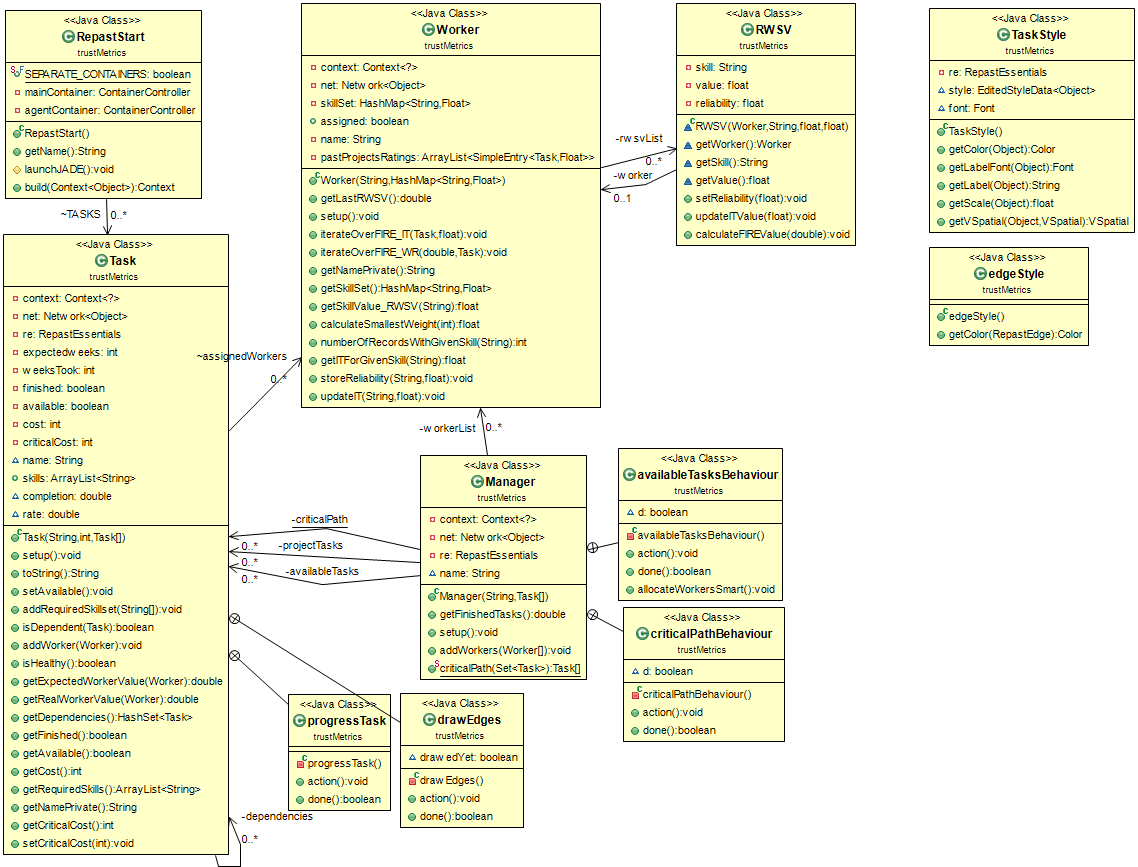
\includegraphics[scale=0.4]{Model.png}
\end{center}

\section{Experiences}
In order to test our model, we defined a project with several tasks with different requirements and dependencies and provided two workers, with a different set of skills and ratings to attend to those tasks. The skill requirements of the Tasks are as follows:
\begin{center}
	$Task A  ->  {C++}$
	\\
	$Task B  ->  {Java}$
	\\
	$Task C  ->  {Java,C++}$
	\\
	$Task D  ->  {Management}$
\end{center}
The workers have the following skill sets and ratings, where -1 is absolutely negative, 0 is neutral and 1 is absolutely positive.
\begin{center}
	$Worker 1  ->  {<C++,1>,<Java,0.5>}$
	\\
	$Worker 2  ->  {<Java,0.5>,<Management,1>}$
\end{center}
We this information set, we can initialize our project and view it on the Repast environment.
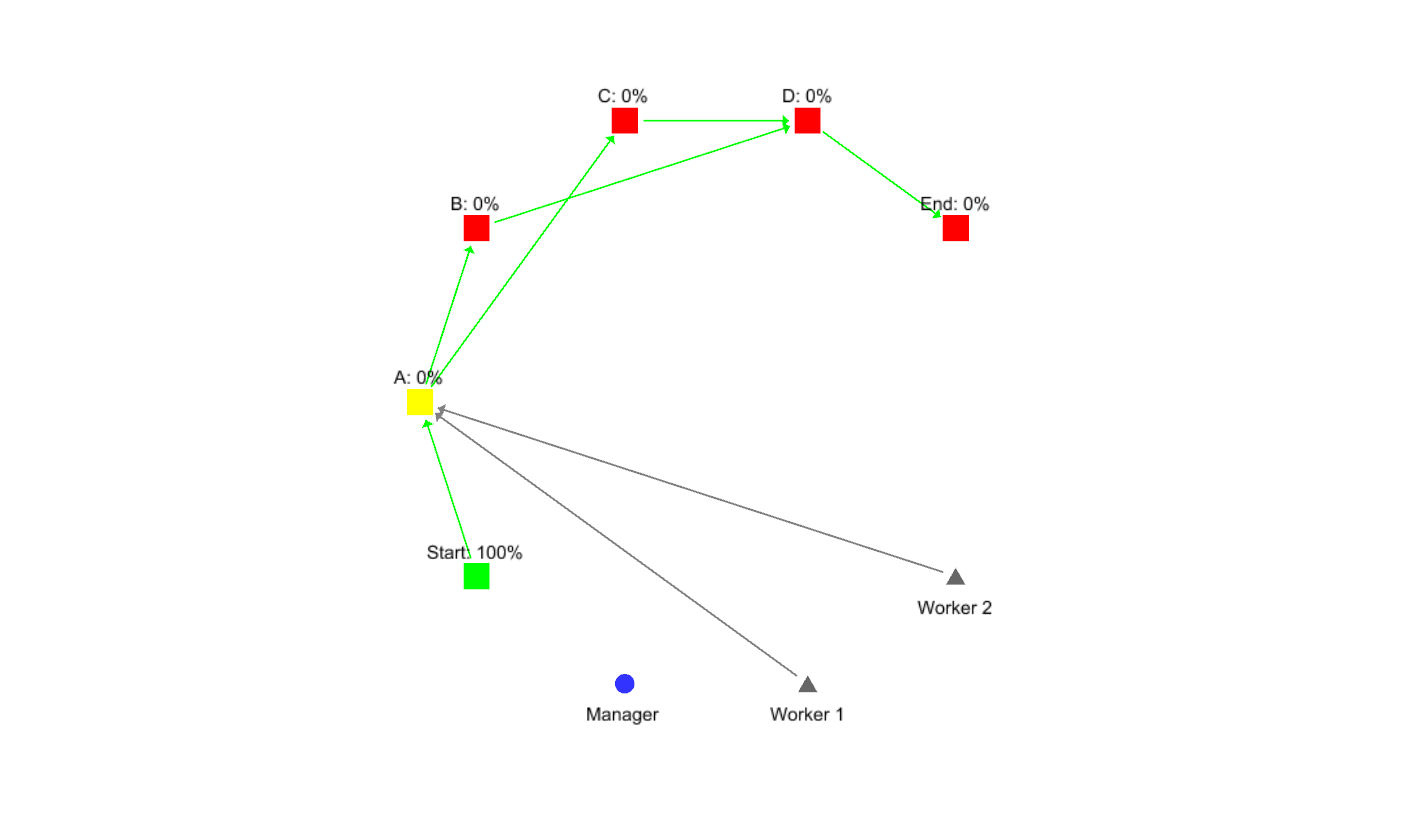
\includegraphics[scale=0.3]{exp1.png}
At the moment we display this image we are at tick count 3 and some things have already happened. For example, the manager has executed his first behaviour, which is to calculate the Critical Path method and order the tasks by critical time. It has also executed its second behaviour, which is to find out if there are any available tasks and assign workers. At the start of the project there is only one available task and the manager assigns both workers to it, since he knows nothing about their skills and he might as well have them working than in an idle state. We will know display the project as soon as Task A finishes.
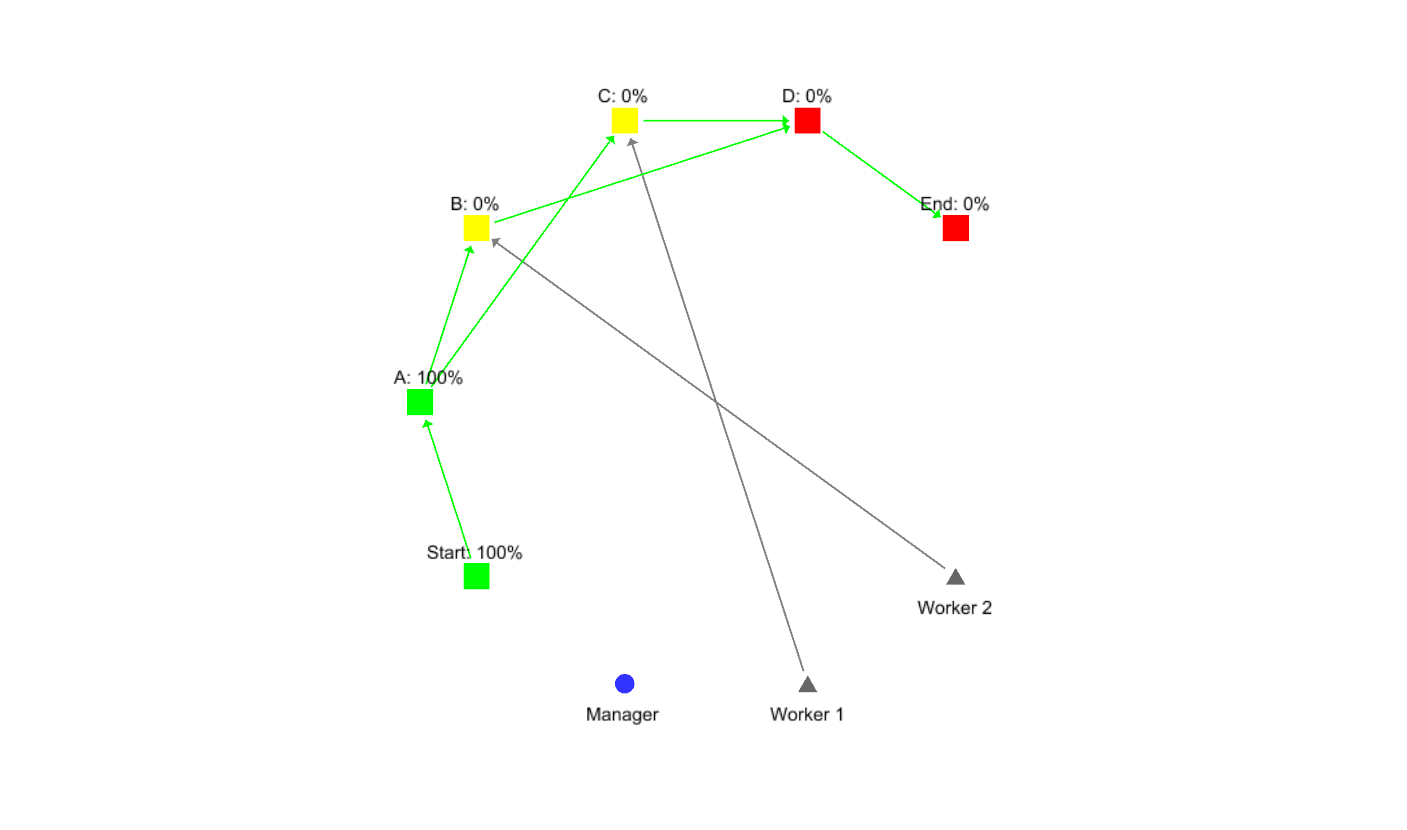
\includegraphics[scale=0.3]{exp2.png}
\begin{center}
	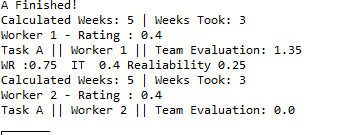
\includegraphics[scale=1]{data1.png}
\end{center}
The first thing we notice is that the first batch of data gathered by the manager about the workers is displayed in the console. Remember that the manager starts by assuming the workers are neutral on all their skills, however, if we take a look at the definition of the workers we can notice they actually have very positive ratings, thus, the task finished sooner than the manager expected and the supposed rating of the workers skills received positive reinforcement.
With the new supposed values the workers skills, the manager will decide the best way to allocate them to the two newly unlocked tasks. Since the value of Worker 1 is sufficient to satisfy the estimated duration of task B and the same happens with Worker 2 and Task C, the manager is able to perform a parallel allocation.

We can follow this process until the end of the project noticing that when a worker is free, he does not stay idle but helps other workers in the remaining tasks, as long as he is minimally useful. We will now fast forward to the end of the project and analyse the final data.

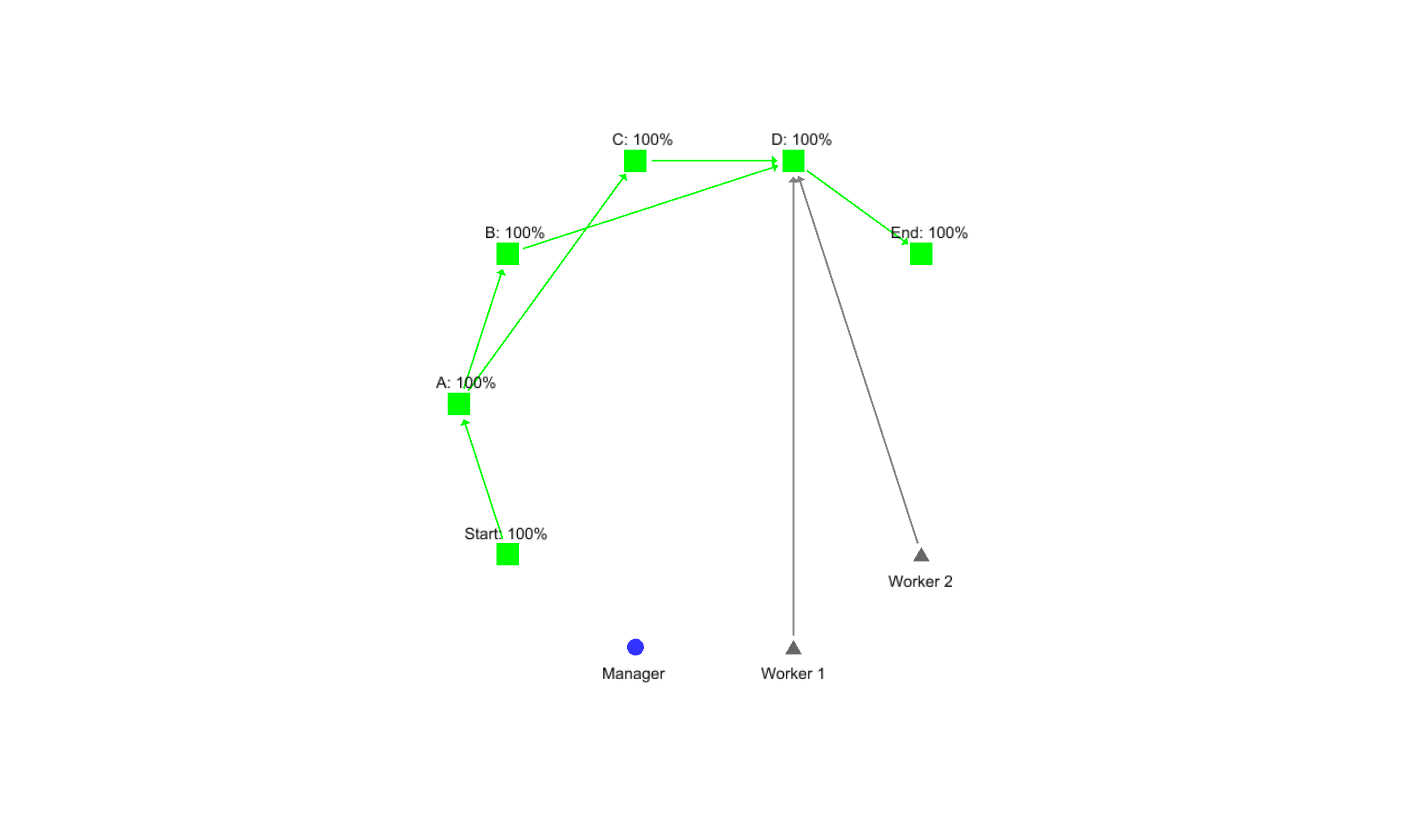
\includegraphics[scale=0.3]{exp3.png}
\begin{center}
	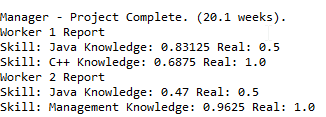
\includegraphics[scale=1]{data2.png}
\end{center}
The project was complete in 20.1 weeks, however, every instance of the same project may have slightly different dates due to random events that may slow or speed up the progress of some tasks. In this instance, we can see that the manager has managed to guess the ratings of Worker 2 quite well while with Worker 2 he is a little more far from the real values. It is important to note the objective of the manager is not to completely know the ratings of the workers, this is merely a means to an end, which is to conclude the project in the shortest amount of time.
\section{Conclusions}

The usage of trust metrics in a system is an expanding area because of its ability to adapt to a shape shifting environment and to question other agents' intentions or usefulness given our own agents' intentions.

Even with all these flexible abilities, trust metrics algorithms like FIRE can still maintain high performance, translated in allowing quite optimal decisions.

In this specific application and with this implementation, FIRE behaved in a way that may begin with some rough, low accuracy, estimations of the real agent value but it displayed a fast evolution leaning close to that real hidden value.
In recognition of the early estimations problem, this implementation takes into account history size and history consistency. With this, the first few interactions are careful and the deviation between real and expected interactions is mitigated.

In a world with an expanding and interactive pool of computational agents and with such an unstable landscape with diverse intentions, solutions and algorithms like this can very well present an optimal solution to develop an agent that works in cooperation with other agents towards its goals in a fast, efficient and trusted way.

\section{Improvement}
It would be interesting to implement other Trust Models in order to compare their different success rates on recognizing worker value, which would of course affect positively the end due to more proper allocation. Another feature that would greatly increase the collection of data and testing of the trust models would be a project generator. Since we manually define the project at start-up it is very time consuming to properly think and implement large projects. A project generator would allow us to create very large projects, with different types and combinations of tasks. This would allow the trust models to measure differentiation in different skill requirements and eventually compute a very close approximation to the real values of the workers skills. Other interesting features would be implementing experience learning (workers increasing their skill values as they work, and manager accounting for that) and manager skill being a factor as well.






\newpage
\begin{thebibliography}{9}
	\bibitem{fire} 
	T. Dong Huynh and Nicholas R. Jennings and Nigel R. Shadbolt
	\textit{FIRE: An Integrated Trust and Reputation Model for
		Open Multi-Agent Systems
}. 

	
	\bibitem{cpm} 
	University of Alabama,
	\\\texttt{http:/www.ctl.ua.edu/{}math103/scheduling/scheduling\_algorithms.html}
\end{thebibliography}
\end{document}
